\section{Premica}

\begin{frame}
    \sectionpage
\end{frame}

\begin{frame}
    \tableofcontents[currentsection, hideothersubsections]
\end{frame}
        


    \subsection{Enačba premice}

        \begin{frame}
            \frametitle{Enačba premice}
        \end{frame}


        \begin{frame}
            \only<2->{\begin{exampleblock}{Naloga}
                Narišite premico z dano eksplicitno obliko enačbe.
                    \begin{itemize}
                        \item $y=-2x+1$
                        \item $y=\dfrac{1}{2}x+2$
                        \item $y=2x+\dfrac{3}{4}$
                    \end{itemize}
            \end{exampleblock}}

            \only<3->{\begin{exampleblock}{Naloga}
                Narišite premico z dano odsekovno obliko enačbe.
                \vskip-1em
                \begin{columns}
                    \column{0.5\textwidth}
                    \begin{itemize}
                        \item $\dfrac{x}{3}+\dfrac{y}{5}=1$
                        \item $\dfrac{x}{2}+\dfrac{2y}{5}=1$
                    \end{itemize}

                    \column{0.47\textwidth}
                    \begin{itemize}
                        \item $\dfrac{x}{2}-\dfrac{y}{4}=1$
                        \item $\dfrac{x}{2}-\dfrac{y}{3}=-1$
                    \end{itemize}
                \end{columns}
            \end{exampleblock}}
        \end{frame}


                \begin{frame}
            \only<2->{\begin{exampleblock}{Naloga}
                Z grafa razberite ničlo in začetno vrednost ter zapišite odsekovno obliko enačbe premice.

                \begin{columns}
                    \column{0.32\textwidth}
                    \vskip-1.5em
                    \begin{figure}[H]
                        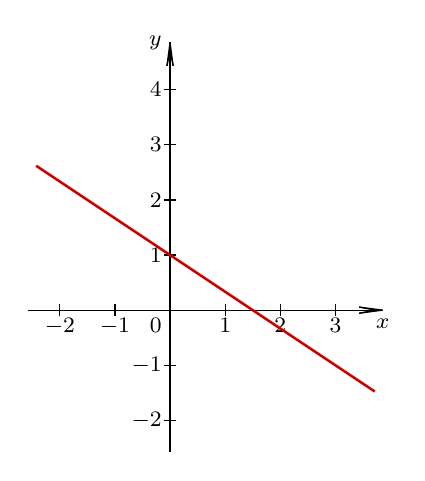
\begin{tikzpicture}
                            % \clip (0,0) rectangle (14.000000,10.000000);
                            {\footnotesize
                            
                            % Drawing 2D Cartesian system
                            \draw (3.000000,3.000000) node [anchor=north east] { $0$ };%
                            \draw [line width=0.016cm] (3.000000,2.925000) -- (3.000000,3.075000);%
                            \draw (3.700000,3.000000) node [anchor=north] { $1$ };%
                            \draw [line width=0.016cm] (3.700000,2.925000) -- (3.700000,3.075000);%
                            \draw (4.400000,3.000000) node [anchor=north] { $2$ };%
                            \draw [line width=0.016cm] (4.400000,2.925000) -- (4.400000,3.075000);%
                            \draw (5.100000,3.000000) node [anchor=north] { $3$ };%
                            \draw [line width=0.016cm] (5.100000,2.925000) -- (5.100000,3.075000);%
                            \draw (2.300000,3.000000) node [anchor=north] { $-1$ };%
                            \draw [line width=0.016cm] (2.300000,2.925000) -- (2.300000,3.075000);%
                            \draw (1.600000,3.000000) node [anchor=north] { $-2$ };%
                            \draw [line width=0.016cm] (1.600000,2.925000) -- (1.600000,3.075000);%
                            \draw (3.000000,3.700000) node [anchor=east] { $1$ };%
                            \draw [line width=0.016cm] (2.925000,3.700000) -- (3.075000,3.700000);%
                            \draw (3.000000,4.400000) node [anchor=east] { $2$ };%
                            \draw [line width=0.016cm] (2.925000,4.400000) -- (3.075000,4.400000);%
                            \draw (3.000000,5.100000) node [anchor=east] { $3$ };%
                            \draw [line width=0.016cm] (2.925000,5.100000) -- (3.075000,5.100000);%
                            \draw (3.000000,5.800000) node [anchor=east] { $4$ };%
                            \draw [line width=0.016cm] (2.925000,5.800000) -- (3.075000,5.800000);%
                            \draw (3.000000,2.300000) node [anchor=east] { $-1$ };%
                            \draw [line width=0.016cm] (2.925000,2.300000) -- (3.075000,2.300000);%
                            \draw (3.000000,1.600000) node [anchor=east] { $-2$ };%
                            \draw [line width=0.016cm] (2.925000,1.600000) -- (3.075000,1.600000);%
                            \draw (5.700000,3.000000) node [anchor=north] { $x$ };%
                            \draw (3.000000,6.400000) node [anchor=east] { $y$ };%
                            \draw [line width=0.016cm] (1.200000,3.000000) -- (5.700000,3.000000);%
                            \draw [line width=0.016cm] (5.402567,3.039158) -- (5.700000,3.000000);%
                            \draw [line width=0.016cm] (5.402567,3.039158) -- (5.600000,3.000000);%
                            \draw [line width=0.016cm] (5.402567,2.960842) -- (5.700000,3.000000);%
                            \draw [line width=0.016cm] (5.402567,2.960842) -- (5.600000,3.000000);%
                            \draw [line width=0.016cm] (3.000000,1.200000) -- (3.000000,6.400000);%
                            \draw [line width=0.016cm] (2.960842,6.102567) -- (3.000000,6.400000);%
                            \draw [line width=0.016cm] (2.960842,6.102567) -- (3.000000,6.300000);%
                            \draw [line width=0.016cm] (3.039158,6.102567) -- (3.000000,6.400000);%
                            \draw [line width=0.016cm] (3.039158,6.102567) -- (3.000000,6.300000);%
                            
                            % Changing color 204 0 0
                            \definecolor{r204g0b0}{rgb}{0.800000,0.000000,0.000000}%
                            \color{r204g0b0}% 
                            
                            % Drawing line l
                            \draw [line width=0.032cm] (1.300000,4.833220) -- (5.600000,1.966840);%
                            \color{black}
                            }
                            \end{tikzpicture}
                                                        
                    \end{figure}

                    \column{0.32\textwidth}
                    \vskip-1.5em
                    \begin{figure}[H]
                        \begin{tikzpicture}
                            % \clip (0,0) rectangle (14.000000,10.000000);
                            {\footnotesize
                            
                            % Drawing 2D Cartesian system
                            \draw (3.000000,3.000000) node [anchor=north east] { $0$ };%
                            \draw [line width=0.016cm] (3.000000,2.925000) -- (3.000000,3.075000);%
                            \draw (3.700000,3.000000) node [anchor=north] { $1$ };%
                            \draw [line width=0.016cm] (3.700000,2.925000) -- (3.700000,3.075000);%
                            \draw (4.400000,3.000000) node [anchor=north] { $2$ };%
                            \draw [line width=0.016cm] (4.400000,2.925000) -- (4.400000,3.075000);%
                            \draw (5.100000,3.000000) node [anchor=north] { $3$ };%
                            \draw [line width=0.016cm] (5.100000,2.925000) -- (5.100000,3.075000);%
                            \draw (2.300000,3.000000) node [anchor=north] { $-1$ };%
                            \draw [line width=0.016cm] (2.300000,2.925000) -- (2.300000,3.075000);%
                            \draw (1.600000,3.000000) node [anchor=north] { $-2$ };%
                            \draw [line width=0.016cm] (1.600000,2.925000) -- (1.600000,3.075000);%
                            \draw (3.000000,3.700000) node [anchor=east] { $1$ };%
                            \draw [line width=0.016cm] (2.925000,3.700000) -- (3.075000,3.700000);%
                            \draw (3.000000,4.400000) node [anchor=east] { $2$ };%
                            \draw [line width=0.016cm] (2.925000,4.400000) -- (3.075000,4.400000);%
                            \draw (3.000000,5.100000) node [anchor=east] { $3$ };%
                            \draw [line width=0.016cm] (2.925000,5.100000) -- (3.075000,5.100000);%
                            \draw (3.000000,5.800000) node [anchor=east] { $4$ };%
                            \draw [line width=0.016cm] (2.925000,5.800000) -- (3.075000,5.800000);%
                            \draw (3.000000,2.300000) node [anchor=east] { $-1$ };%
                            \draw [line width=0.016cm] (2.925000,2.300000) -- (3.075000,2.300000);%
                            \draw (3.000000,1.600000) node [anchor=east] { $-2$ };%
                            \draw [line width=0.016cm] (2.925000,1.600000) -- (3.075000,1.600000);%
                            \draw (5.700000,3.000000) node [anchor=north] { $x$ };%
                            \draw (3.000000,6.400000) node [anchor=east] { $y$ };%
                            \draw [line width=0.016cm] (1.200000,3.000000) -- (5.700000,3.000000);%
                            \draw [line width=0.016cm] (5.402567,3.039158) -- (5.700000,3.000000);%
                            \draw [line width=0.016cm] (5.402567,3.039158) -- (5.600000,3.000000);%
                            \draw [line width=0.016cm] (5.402567,2.960842) -- (5.700000,3.000000);%
                            \draw [line width=0.016cm] (5.402567,2.960842) -- (5.600000,3.000000);%
                            \draw [line width=0.016cm] (3.000000,1.200000) -- (3.000000,6.400000);%
                            \draw [line width=0.016cm] (2.960842,6.102567) -- (3.000000,6.400000);%
                            \draw [line width=0.016cm] (2.960842,6.102567) -- (3.000000,6.300000);%
                            \draw [line width=0.016cm] (3.039158,6.102567) -- (3.000000,6.400000);%
                            \draw [line width=0.016cm] (3.039158,6.102567) -- (3.000000,6.300000);%
                            
                            % Changing color 204 0 0
                            \definecolor{r204g0b0}{rgb}{0.800000,0.000000,0.000000}%
                            \color{r204g0b0}% 
                            
                            % Drawing line l
                            \draw [line width=0.032cm] (2.700000,1.300000) -- (5.600000,4.200000);%
                            \color{black}
                            }
                            \end{tikzpicture}
                            
                    \end{figure}

                    \column{0.32\textwidth}
                    \vskip-1.5em
                    \begin{figure}[H]
                        \begin{tikzpicture}
                            % \clip (0,0) rectangle (14.000000,10.000000);
                            {\footnotesize
                            
                            % Drawing 2D Cartesian system
                            \draw (3.000000,3.000000) node [anchor=north east] { $0$ };%
                            \draw [line width=0.016cm] (3.000000,2.925000) -- (3.000000,3.075000);%
                            \draw (3.700000,3.000000) node [anchor=north] { $1$ };%
                            \draw [line width=0.016cm] (3.700000,2.925000) -- (3.700000,3.075000);%
                            \draw (4.400000,3.000000) node [anchor=north] { $2$ };%
                            \draw [line width=0.016cm] (4.400000,2.925000) -- (4.400000,3.075000);%
                            \draw (5.100000,3.000000) node [anchor=north] { $3$ };%
                            \draw [line width=0.016cm] (5.100000,2.925000) -- (5.100000,3.075000);%
                            \draw (2.300000,3.000000) node [anchor=north] { $-1$ };%
                            \draw [line width=0.016cm] (2.300000,2.925000) -- (2.300000,3.075000);%
                            \draw (1.600000,3.000000) node [anchor=north] { $-2$ };%
                            \draw [line width=0.016cm] (1.600000,2.925000) -- (1.600000,3.075000);%
                            \draw (3.000000,3.700000) node [anchor=east] { $1$ };%
                            \draw [line width=0.016cm] (2.925000,3.700000) -- (3.075000,3.700000);%
                            \draw (3.000000,4.400000) node [anchor=east] { $2$ };%
                            \draw [line width=0.016cm] (2.925000,4.400000) -- (3.075000,4.400000);%
                            \draw (3.000000,5.100000) node [anchor=east] { $3$ };%
                            \draw [line width=0.016cm] (2.925000,5.100000) -- (3.075000,5.100000);%
                            \draw (3.000000,5.800000) node [anchor=east] { $4$ };%
                            \draw [line width=0.016cm] (2.925000,5.800000) -- (3.075000,5.800000);%
                            \draw (3.000000,2.300000) node [anchor=east] { $-1$ };%
                            \draw [line width=0.016cm] (2.925000,2.300000) -- (3.075000,2.300000);%
                            \draw (3.000000,1.600000) node [anchor=east] { $-2$ };%
                            \draw [line width=0.016cm] (2.925000,1.600000) -- (3.075000,1.600000);%
                            \draw (5.700000,3.000000) node [anchor=north] { $x$ };%
                            \draw (3.000000,6.400000) node [anchor=east] { $y$ };%
                            \draw [line width=0.016cm] (1.200000,3.000000) -- (5.700000,3.000000);%
                            \draw [line width=0.016cm] (5.402567,3.039158) -- (5.700000,3.000000);%
                            \draw [line width=0.016cm] (5.402567,3.039158) -- (5.600000,3.000000);%
                            \draw [line width=0.016cm] (5.402567,2.960842) -- (5.700000,3.000000);%
                            \draw [line width=0.016cm] (5.402567,2.960842) -- (5.600000,3.000000);%
                            \draw [line width=0.016cm] (3.000000,1.200000) -- (3.000000,6.400000);%
                            \draw [line width=0.016cm] (2.960842,6.102567) -- (3.000000,6.400000);%
                            \draw [line width=0.016cm] (2.960842,6.102567) -- (3.000000,6.300000);%
                            \draw [line width=0.016cm] (3.039158,6.102567) -- (3.000000,6.400000);%
                            \draw [line width=0.016cm] (3.039158,6.102567) -- (3.000000,6.300000);%
                            
                            % Changing color 204 0 0
                            \definecolor{r204g0b0}{rgb}{0.800000,0.000000,0.000000}%
                            \color{r204g0b0}% 
                            
                            % Drawing line l
                            \draw [line width=0.032cm] (4.900000,6.300000) -- (1.300000,2.700000);%
                            \color{black}
                            }
                            \end{tikzpicture}
                            
                    \end{figure}

                \end{columns}

            \end{exampleblock}}

        \end{frame}


        \begin{frame}
            \only<2->{\begin{exampleblock}{Naloga}
                Dano enačbo premice zapišite v eksplicitni in odsekovni obliki ter premico narišite.
                \vskip-1em
                \begin{columns}
                    \column{0.5\textwidth}
                    \begin{itemize}
                        \item $x+4y-8=0$
                        \item $3x-2y+6=0$
                        \item $2x+5y+5=0$
                    \end{itemize}

                    \column{0.47\textwidth}
                    \begin{itemize}
                        \item $\dfrac{1}{2}x+3y-6=0$
                        \item $x+1=0$
                        \item $y-2=0$ \\~
                    \end{itemize}
                \end{columns}

            \end{exampleblock}}

            \only<3->{\begin{exampleblock}{Naloga}
                Izračunajte ploščino trikotnika, ki jo premica oklepa s koordinatnima osema.
                \vskip-1em
                \begin{columns}
                    \column{0.5\textwidth}
                    \begin{itemize}
                        \item $y=-2x+4$
                        \item $\dfrac{x}{2}+\dfrac{x}{-3}=1$
                    \end{itemize}

                    \column{0.47\textwidth}
                    \begin{itemize}
                        \item $2x+4y-3=0$
                        \item $x-y+1=0$ \\~
                    \end{itemize}
                \end{columns}
            \end{exampleblock}}

        \end{frame}


        \begin{frame}
            \only<2->{\begin{exampleblock}{Naloga}
                Zapišite enačbo premice, ki gre skozi dani točki.
                    \begin{itemize}
                        \item $A(2,3)$ in $B(4,5)$ 
                        \item $C(1,-2)$ in $D(-3,-4)$ 
                        \item $E(7,2)$ in $F(-7,-5)$ \\~
                    \end{itemize}
            \end{exampleblock}}

            \only<3->{\begin{exampleblock}{Naloga}
                Določite neznano koordinato tako, da bodo dane točke kolinearne.
                    \begin{itemize}
                        \item $A(3,y)$, $B(-4,1)$ in $C(2,2)$ 
                        \item $D(-1,7)$, $E(x,5)$ in $F(3,-4)$ \\~
                    \end{itemize}
            \end{exampleblock}}

        \end{frame}


        \begin{frame}
            \only<2->{\begin{exampleblock}{Naloga}
                Ugotovite, ali sta dani premici vzporedni.
                    \begin{itemize}
                        \item $y=\dfrac{3}{4}x-1$ in $y=-\dfrac{3}{4}x+1$ \\~
                        \item $x-2y+1=0$ in $2x+y+1=0$ \\~
                        \item $\dfrac{x}{3}-\dfrac{y}{6}=1$ in $\dfrac{x}{2}+\dfrac{y}{4}=1$ \\~
                        \item $\dfrac{x}{4}+\dfrac{y}{2}=1$ in $4x+2y+1=0$ \\~

                    \end{itemize}
            \end{exampleblock}}


        \end{frame}


        \begin{frame}
            
            \only<2->{\begin{exampleblock}{Naloga}
                Dani sta premici z enačbama $y=4x+9$ in $ax-3y+3=0$. Določite parameter $a$ tako, da bosta premici vzporedni.
            \end{exampleblock}}

            \only<3->{\begin{exampleblock}{Naloga}
                Dani sta premici z enačbama $\dfrac{x}{2}-\dfrac{y}{7}=1$ in $-6x+by+1=0$. Določite parameter $b$ tako, da bosta premici vzporedni.
            \end{exampleblock}}

            \only<4->{\begin{exampleblock}{Naloga}
                Dani sta premici z enačbama $3x-2y+4=0$ in $(c-2)x+4y+3=0$. Določite parameter $c$ tako, da bosta premici vzporedni.
            \end{exampleblock}}

        \end{frame}


        \begin{frame}
            \only<2->{\begin{exampleblock}{Naloga}
                Zapišite enačbo premice, ki je vzporedna dani premici in poteka skozi dano točko.
                    \begin{itemize}
                        \item $y=2x-1$, $T(1,-3)$ 
                        \item $2x-4y+3=0$, $U(-4,5)$ 
                        \item $\dfrac{x}{4}+\dfrac{y}{8}=1$, $V(8,-8)$ \\~

                    \end{itemize}
            \end{exampleblock}}


            \only<3->{\begin{exampleblock}{Naloga}
                Iz snopa premic z enačbo $y=-3x+n$ določite enačbo tiste premice, ki poteka skozi točko $(1,4)$.
            \end{exampleblock}}

            \only<4->{\begin{exampleblock}{Naloga}
                Iz šopa premic z enačbo $y=kx+2$ določite enačbo tiste premice, ki gre skozi točko $(3,-4)$.
            \end{exampleblock}}

        \end{frame}


        \begin{frame}
            \only<2->{\begin{exampleblock}{Naloga}
                Zapišite enačbo pravokotnice na dano premico, ki poteka skozi dano točko.
                    \begin{itemize}
                        \item $y=x+2$, $T(3,-4)$ \\~
                        \item $y=2x+3$, $U(4,5)$ \\~
                        \item $y=\dfrac{1}{3}x+5$, $V(-1,4)$ \\~
                        \item $y=-\dfrac{2}{3}x+\dfrac{4}{5}$, $Z(-6,3)$ \\~

                    \end{itemize}
            \end{exampleblock}}

        \end{frame}




    \subsection{Presešišče premic}

        \begin{frame}
            \frametitle{Presešišče premic}
        \end{frame}


